\documentclass[fleqn]{article}
\usepackage[english]{babel}
\usepackage{a4wide}
\usepackage{latexsym}
\usepackage{times}
%\usepackage{theorem}
\usepackage{url}
\usepackage[final]{graphics}
\usepackage{amsmath,amssymb}
\usepackage{amsfonts}
\usepackage{array}
\usepackage{calc}
\usepackage{xspace}
\usepackage{color}
\usepackage{epsfig}
\usepackage{subfigure}
\usepackage{float}
\usepackage{stmaryrd}
\usepackage{color}
\usepackage{mathtools}
\usepackage{graphicx}
\usepackage{epstopdf}
\usepackage{listings}
\usepackage{color}
\usepackage{booktabs,caption}
%\usepackage[flushleft]{threeparttable}
%\usepackage{amsmath}
\DeclareMathAlphabet{\mathpzc}{OT1}{pzc}{m}{it}
\usepackage{amsthm,amssymb}

\usepackage{amssymb}
\usepackage{graphicx}
\usepackage{epstopdf}
\usepackage{mathtools}

\usepackage{algorithm}
\usepackage[noend]{algpseudocode}

\usepackage{fouriernc}
\pagestyle{plain}
\usepackage{float}
\usepackage[hidelinks]{hyperref}

\usepackage{array}
\newcolumntype{L}[1]{>{\raggedright\let\newline\\\arraybackslash\hspace{0pt}}m{#1}}
\newcolumntype{C}[1]{>{\centering\let\newline\\\arraybackslash\hspace{0pt}}m{#1}}
\newcolumntype{R}[1]{>{\raggedleft\let\newline\\\arraybackslash\hspace{0pt}}m{#1}}

\newtheorem{theorem}{Theorem}
\newtheorem{corollary}{Corollary}
\newtheorem{fact}{Fact}
\newtheorem{hypothesis}{Hypothesis}
\newtheorem{lemma}{Lemma}
\newtheorem{definition}{Definition}

\definecolor{codegreen}{rgb}{0,0.6,0}
\definecolor{codegray}{rgb}{0.5,0.5,0.5}
\definecolor{codepurple}{rgb}{0.58,0,0.82}
\definecolor{backcolour}{rgb}{0.95,0.95,0.92}

\lstdefinestyle{mystyle}{
	backgroundcolor=\color{backcolour},   
	commentstyle=\color{codegreen},
	keywordstyle=\color{magenta},
	numberstyle=\tiny\color{codegray},
	stringstyle=\color{codepurple},
	basicstyle=\footnotesize,
	breakatwhitespace=false,         
	breaklines=true,                 
	captionpos=b,                    
	keepspaces=true,                 
	numbers=left,                    
	numbersep=5pt,                  
	showspaces=false,                
	showstringspaces=false,
	showtabs=false,                  
	tabsize=2
}

\lstset{style=mystyle}


\usepackage{fouriernc}
\pagestyle{plain}

%% macros.tex

\title{\sf Towards BCRT for FPTS\\
			Exact analysis}
\author{{\sf H.J. Rivera Verduzco 0977393}\\
{\footnotesize\sl P.O.~Box 513, 5600 MB Eindhoven, The Netherlands}\\
{\footnotesize \sl Email: \tt H.J.Rivera.Verduzco@student.tue.nl}}
%\date{}
\begin{document}
\maketitle

%\begin{abstract}
%\noindent
% Add abstract here %
%\end{abstract}

\section{Exact best-case analysis for FPTS}

\subsection{Optimal instant}
Based on Fact 3, we can distinguish between two types of tasks than can influence the \textit{best-case response time} of a task $\tau_i$. These types of tasks are the set of \textit{preemptive} tasks $\mathpzc{H_i}=\{\tau_h | \pi_h>\theta_i\}$, and the set of \textit{delaying} tasks $\mathpzc{D_i}=\{\theta_i \geq \pi_d > \pi_i\}$. Furthermore, Fact 5 shows that for some cases the \textit{best-case response time} of a task $\tau_i$ is not necessarily found in the job experiencing the \textit{best-case hold time}. Therefore, the activation of all \textit{preemptive} tasks may not coincide with the completion of the job $k^{bcrt}$ of $\tau_i$ that assumes the \textit{best-case response time}. Instead, some \textit{preemptive} tasks may give rise to extra preemptions in $k^{bcrt}$ in order to increase the \textit{hold time} $H_{i,k^{bcrt}}$ and subsequently reduce the \textit{response time} $R_{i,k^{bcrt}}$. Based on the previous observation, we divide the set of \textit{preemptive} tasks $\mathpzc{H_i}$ of a task $\tau_i$  into the set of \textit{preemptive} tasks that give rise to extra preemptions denoted as $\mathpzc{E_i} \subseteq \mathpzc{H_i}$, and the remaining preemptive tasks that we call \textit{best preemptive} tasks in the set $\mathpzc{P_i}=\mathpzc{H_i}\backslash\mathpzc{E_i}$.

We now formulate the notion of optimal instant for FPTS based on the set of tasks influencing the \textit{best-case response time} of a task $\tau_i$.

\begin{theorem} \label{thm:optimal_instant_fpts}
	In FPTS, an optimal instant for a task $\tau_i$ occurs when the completion of a job $\iota_{i,k}$ of $\tau_i$ coincides with a simultaneous activation of all \textit{best preemptive} tasks $\tau_p\in\mathpzc{P_i}$. Furthermore, the activation of all delaying tasks $\tau_d \in \mathpzc{D_i}$ and all \textit{extra preemptive} tasks $\tau_e \in \mathpzc{E_i}$, coincides with $s_{i,k}+\Delta$, where $\Delta$ is a sufficiently small amount of time 
\end{theorem}

Note that, given a task-set $\mathpzc{T}$ and a task $\tau_i \in \mathpzc{T}$, the set of \textit{delaying} tasks $\mathpzc{D_i}$ is empty when the preemption-threshold of $\tau_i$ is equal to its priority. Furthermore, the set of \textit{extra preemptive} tasks $\mathpzc{E_i}$ is always empty when there are no \textit{delaying} tasks. Therefore, we conclude that the optimal instant for a task $\tau_i$ scheduled under FPTS described in Theorem \ref{thm:optimal_instant_fpts} specializes to an optimal instant for FPPS when $\theta_i = \pi_i$ . 

Figure \ref{fig:optimal_instant} shows an example of an optimal instant under FPTS for task $\tau_i$ of the task-set $\mathpzc{T}_{\ref{tab:ex_opt_instant}}$ described in Table \ref{tab:ex_opt_instant}. As can be seen, the activation of the \textit{best preemptive} task $\tau_{h1}$ coincides with the completion of task $\tau_i$ at time $t=0$. Furthermore, \textit{delaying} task $\tau_d$ and \textit{extra} preemptive task $\tau_{h2}$ are activated an instant $\Delta$ after the start of $\tau_i$.

\begin{table}[H]
	\center
	\caption{Characteristics of task-set $\mathpzc{T}_{\ref{tab:ex_opt_instant}}$.}
	\label{tab:ex_opt_instant}
	\begin{tabular}{c c c c c | c}
		\hline 
		& $T_i$ & $C_i$ & $\pi_i$ & $\theta_i$ & $BR_i$\\ 
		\hline 
		$\tau_{h1}$& 35 & 5  & 4 & 4 & 5\\ 
		$\tau_{h2}$& 35 & 5  & 3 & 3 & 5\\ 
		$\tau_d$& 50 & 20 & 2 & 2 & 20\\ 
		$\tau_i$& 70 & 22 & 1 & 2 & 27\\
		\hline 
	\end{tabular}
	\small
	\item The \textit{least common multiple} of the periods is 350 and $U^{\mathpzc{T_{\ref{tab:ex_opt_instant}}}}=1$.
\end{table}

\begin{figure}[H]
	\centering
	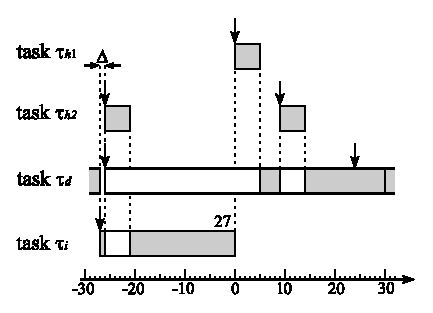
\includegraphics[width=0.55\linewidth]{figures/optimal_instant1}
	\caption{Optimal instant for task $\tau_i\in \mathpzc{T}_{\ref{tab:ex_opt_instant}}$ under FPTS when $\mathpzc{E}_i = \{\tau_{h2}\}$ and $\mathpzc{P}_i = \{\tau_{h1}\}$. }
	\label{fig:optimal_instant}
\end{figure}

It is worth noting that, from the notion of optimal instant given above, it is not clear whether a \textit{preemptive} task should belong to the set of \textit{extra preemptive} tasks or to the set of \textit{best preemptive} tasks. In fact, we could have chosen $\mathpzc{E_i}=\{\tau_{h1}\}$ and $\mathpzc{P_i}=\{\tau_{h2}\}$ in the example depicted in Figure \ref{fig:optimal_instant}, and we would still have obtained an option that is in accordance with the notion of optimal instant given in Theorem \ref{thm:optimal_instant_fpts}. Therefore, we can conclude that in FPTS there may be multiple candidates of optimal instants that we have to explore in order to find the \textit{best-case response time} of a task $\tau_i$. In the worst of the cases, these candidates of optimal instant are determined based on all possible combinations of \textit{extra preemptive} and \textit{best preemptive} tasks. Clearly, this differs from the best-case analysis for FPPS, where the optimal instant is always unique.

% rise to different candidate instants where the best-case response time can be found. For instance, if there are two \textit{preemptive} tasks that can preempt a task $\tau_i$, there are four candidates of optimal instants. Those are when 

%It is worth noting that the notion of optimal instant given above gives rise to different candidate instants where the best-case response time can be found. For instance, if there are two \textit{preemptive} tasks that can preempt a task $\tau_i$, there are four candidates of optimal instants. Those are when 

\subsection{Determining the phasing of delaying and extra preemptive tasks}
Assuming that we know the set of \textit{extra preemptive} (and \textit{best preemptive}) tasks that lead to the optimal instant where the \textit{best-case response time} for a task $\tau_i$ is found, we now are interested in determining the phasing for each task in order to calculate such a \textit{best-case response time}. According to Theorem \ref{thm:optimal_instant_fpts}, the simultaneous activation of \textit{best-preemptive} tasks has to take place at time $t_1=f_{i,k^{bcrt}}$, where $k^{bcrt}$ is the job of $\tau_i$ that assumes the best-case response time. Furthermore, the simultaneous activation of \textit{delaying} and \textit{extra preemptive} tasks occurs at time $t_2=s_{i,k^{bcrt}}+\Delta$. Therefore, the phasing $\phi_r$ for \textit{delaying} and \textit{extra preemptive} tasks relative to the activation of \textit{best-preemptive} tasks is given by
\begin{align*}
	\phi_r = t_2 - t_1 = (s_{i,k^{bcrt}}+\Delta) - f_{i,k^{bcrt}} = -H_{i,k^{bcrt}}+\Delta.
\end{align*}

We therefore have to determine hold-time $H_{i,k^{bcrt}}$ to derive the proper phasing for \textit{delaying} and \textit{extra preemptive} tasks where we can find the \textit{best-case response time} of task $\tau_i$. Furthermore, note that $H_{i,k^{bcrt}}$ is only influenced by \textit{preemptive} tasks in $\mathpzc{E}_i$ and $\mathpzc{P}_i$ because \textit{delaying tasks} cannot preempt $\tau_i$. In the rest of this section, we introduce the notions of \textit{worst-case} and \textit{best-case} hold intervals. In addition, we determine the hold time $H_{i,k^{bcrt}}$ based on such notions.

\begin{definition}
	The \textit{worst-case hold interval} $WI_i(y,\mathpzc{E})$ is defined as the worst-case hold time of an artificial task $\tau^{\prime}_i$ with computation time of $y \in \mathbb{R}^+$ in task-set $\mathpzc{E}\cup \{\tau^{\prime}_i\}$ given that all jobs in the interval assume their \textit{best-case computation times}.
\end{definition}

The \textit{worst-case hold interval} follows directly from the formula for \textit{worst-case hold time} for FPTS given in \cite{BAHDB17}. The only difference is that best-case computation times are assumed for the \textit{worst-case hold interval}. Hence, $WI_i(y,\mathpzc{E})$ is given by the smallest $x \in \mathbb{R}^+$ satisfying
\begin{align}
x = y + \sum\limits_{e:\pi_e > \theta_i, \tau_e \in \mathpzc{E}}\Big\lceil  \dfrac{x}{T_e}\Big\rceil  BC_e.
\end{align}

\begin{definition} \label{def:best_case_interval}
	The \textit{best-case hold interval} $BI_i(y,\mathpzc{P})$ is defined as the best-case hold time of an artificial task $\tau^{\prime}_i$ with computation time of $y \in \mathbb{R}^+$ in task-set $\mathpzc{P}\cup \{\tau^{\prime}_i\}$ given that $\mathpzc{P}$ contains only preemptive tasks.
	
%	as the length of the shortest interval in which an amount of time $y \in \mathbb{R}^+$ is available for the execution of $\tau_i$ in a task-set $\mathpzc{T}$ scheduled under FPPS. 
\end{definition}

Since Definition \ref{def:best_case_interval} assumes that $\mathpzc{P}$ only contains \textit{preemptive} tasks, we can use the same formula for\textit{ best-case hold time} for FPPS given in \cite{BFV08} to calculate $BI_i(y,\mathpzc{P})$. Hence, function $BI_i(y,\mathpzc{P})$ returns the largest positive solution of $x \in \mathbb{R}^+$ satisfying
\begin{align}
x = y + \sum\limits_{p:\pi_p > \theta_i, \tau_p \in \mathpzc{P}} \Big( \Big\lceil  \dfrac{x}{T_p}\Big\rceil -1 \Big)^+  BC_p.
\end{align}

Finally, we introduce a function to determine the hold-time of a task $\tau_i$ based on its \textit{extra preemptive} and \textit{best-preemptive} tasks.

\begin{definition} \label{def:ht}
	The hold time $HT_i(\mathpzc{E})$ is defined as the shortest hold time of a job $\iota_{i,k}$ of $\tau_i\in \mathpzc{T}$ when experiencing extra preemptions by the tasks in $\mathpzc{E} \subset \mathpzc{T}$. This is, when the tasks in $\mathpzc{E}$ are simultaneously activated at time $s_{i,k}+\Delta$. Where $\Delta$ is a sufficiently small amount of time.  Furthermore, delaying tasks of $\tau_i$ in $ \mathpzc{T}$ are ignored.
\end{definition}

$HT_i(\mathpzc{E})$ is given by the following equation.
\begin{align}
	HT_i(\mathpzc{E}) = \beta_p + \beta_e + BC_i,
\end{align}
where $\beta_p,\beta_e \in \mathbb{R^+} \cup \{0\}$ are the influence that \textit{best preemptive} and \textit{extra preemptive} tasks of $\tau_i$ have in its hold time respectively. The values of $\beta_p$ and $\beta_e$ are given by the smallest solution of the following recursive equations:
\begin{flalign}
\begin{split}
	\beta_e = WI_i(\beta_p+ BC_i,\mathpzc{E}) - \beta_p - BC_i,\\
	\beta_p = BI_i(\beta_e + BC_i,\mathpzc{P}) - \beta_e- BC_i,
\end{split}
\end{flalign}
where $\mathpzc{P} = \{\tau_p | \pi_p > \theta_i, t_p \notin \mathpzc{E}\}$ is the set of \textit{best preemptive} tasks.  $\beta_p$ and $\beta_e$ can be found by an iterative procedure starting with a lower bound.

%\begin{definition}
%	Given a job $\iota_{i,k}$ of a task $\tau_i$ with a hold time $H_{i,k}=HT_i(\mathpzc{E})$, where $\mathpzc{E}$ is a set of \textit{extra preemptive} tasks, the \textit{general best-case interval} $GI_i(y,  \mathpzc{E})$ is defined as the length of the shortest interval before the completion of $\iota_{i,k}$ in which an amount of time $y \in \mathbb{R}^+$ is available for the execution of $\tau_i$.
%\end{definition}

Figure \ref{fig:ht_ex1} shows a timeline depicting $HT_i(\mathpzc{E})=14$ for $\tau_i\in \mathpzc{T}_2$ with characteristics as described in Table \ref{tab:ht_ex1}. As can be seen, task $\tau_e$ is selected as the \textit{extra preemptive} task, i.e. $\mathpzc{E}=\{\tau_e\}$, while $\tau_p$ is a \textit{best preemptive} task. Note that an activation of $\tau_p$ coincides with the completion of the job of $\tau_i$; therefore, minimizing its influence on the hold time of $\tau_i$. In addition, since tasks $\tau_e$ and $\tau_p$ preempt task $\tau_i$ three times each, $\beta_e=6$ and $\beta_p=3$. Finally, note that \textit{delaying} task $\tau_d$ is not considered in Figure \ref{fig:ht_ex1} because Definition \ref{def:ht} assumes that \textit{delaying }tasks are ignored.

\begin{table}[H]
	\center
	\caption{Characteristics of task-set $\mathpzc{T}_{\ref{tab:ht_ex1}}$.}
	\label{tab:ht_ex1}
	\begin{tabular}{c c c c c }
		\hline 
		& $T_i$ & $C_i$ & $\pi_i$ & $\theta_i$\\ 
		\hline 
		$\tau_{p}$& 4 & 1  & 4 & 4 \\ 
		$\tau_{e}$& 5 & 2  & 3 & 3 \\ 
		$\tau_d$& 10 & 1 & 2 & 2 \\ 
		$\tau_i$& 20 & 5 & 1 & 2 \\
		\hline 
	\end{tabular}
	\small
	\item The \textit{least common multiple} of the periods is 20 and $U^{\mathpzc{T_{\ref{tab:ht_ex1}}}}=1$.
\end{table}

\begin{figure}[H]
	\centering
	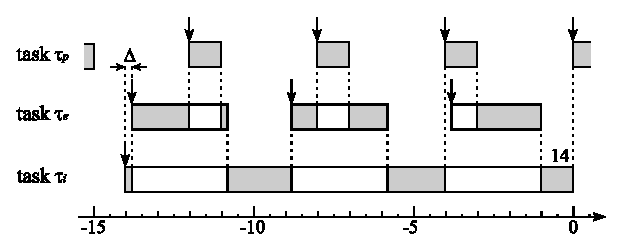
\includegraphics[width=0.7\linewidth]{figures/ht_ex1}
	\caption{Timeline for $\mathpzc{T}_{\ref{tab:ht_ex1}}\backslash\{\tau_d\}$ depicting a job of task $\tau_i$ that assumes a hold time of $HT_i(\mathpzc{E}_i)=14$ where $\mathpzc{E_i} = \{\tau_e\}$. For this example, $\beta_e = 6$ and $\beta_p = 3$.}
	\label{fig:ht_ex1}
\end{figure}

We now formulate a corollary for the phasing $\phi_r$ of \textit{delaying} and \textit{extra preemptive} tasks, based on the hold time of the job of task $\tau_i$ experiencing the optimal instant.

\begin{corollary} \label{col:relative_phasing}
	Let $\mathpzc{E}^{br}_i$ be the set of \textit{extra preemptive} tasks of a task $\tau_i$ that leads to its best-case response time. The phasing of delaying and extra preemptive tasks relative to the activation of best preemptive tasks that leads to an optimal instant is then given by $\phi_r = -HT(\mathpzc{E}^{br}_i)+\Delta$.
\end{corollary}


\subsection{Best-case response time for FPTS}
Similar to the \textit{best-case response time} analysis with arbitrary deadlines for FPPS, a job of a task $\tau_i$ scheduled under FPTS and experiencing its optimal instant may still experience interference by its previous jobs. Therefore, we have to look to previous jobs of task $\tau_i$ to determine its \textit{best-case response time}. In order to do so,  we have to determine intervals of minimal length with enough processing time to execute complete jobs of $\tau_i$.

\begin{definition}
%	The \textit{general best-case interval} $GI_i(y,\mathpzc{E})$ is defined as the length of the shortest interval $[t_s,t_e)$ in which an amount of time $y \in \mathbb{R}^+$ is available for the execution of $\tau_i$ assuming that delaying tasks experience an artificial activation jitter of $\alpha = HT_i(\mathpzc{E})$, and extra preemptive tasks  in $\mathpzc{E}$ are activated at time $t_e-\alpha+\Delta$. Furthermore, all tasks are scheduled under FPPS.
	Given a job $\iota_{i,k}$ of a task $\tau_i$ with a hold time $H_{i,k}=HT_i(\mathpzc{E_i})$, where $\mathpzc{E_i}$ is a set of \textit{extra preemptive} tasks, the \textit{generalized best-case interval} $GI_i(y,  \mathpzc{E_i})$ is defined as the length of the shortest interval before the completion of $\iota_{i,k}$ in which an amount of time $y \in \mathbb{R}^+$ is available for the execution of $\tau_i$.
\end{definition}

Note that $GI_i(y,  \mathpzc{E_i})$ is similar to the notion of \textit{best-case interval} given in \cite{BLM13}. The main difference is that, for $GI_i(y,  \mathpzc{E_i})$, the interval is considered before the completion of a job of $\tau_i$ with hold time $HT_i(\mathpzc{E_i})$. It is necessary to specify the hold time in order to know the phasing at which \textit{extra preemptive} and \textit{delaying} tasks must be activated. Therefore, we propose the following corollary.

\begin{corollary}
	The \textit{generalized best-case interval} $GI_i(y,  \mathpzc{E_i})$ is given by the largest $x \in \mathbb{R}^+$ satisfying

\begin{align} \label{eq:g_best_interval}
%x = y + \sum\limits_{p:\pi_p > \theta_i, \tau_p \notin \mathpzc{E}} \Big( \Big\lceil  \dfrac{x}{T_p}\Big\rceil -1 \Big)^+  BC_p + 
%\sum\limits_{e:\tau_e \in \mathpzc{E}} \Big( \Big\lfloor  \dfrac{x -\alpha}{T_e}\Big\rfloor + \Big\lceil \dfrac{\alpha}{T_e} \Big\rceil \Big) BC_e +
%\sum\limits_{d:\theta_i \geq \pi_d > \pi_i} \Big\lfloor  \dfrac{x-\alpha}{T_d}\Big\rfloor  BC_d,
x = y + \sum\limits_{p:\tau_p \in \mathpzc{P_i}} \Big( \Big\lceil  \dfrac{x}{T_p}\Big\rceil -1 \Big)^+  BC_p +
\sum\limits_{\epsilon:\tau_{\epsilon} \in \mathpzc{E_i} \cup \mathpzc{D_i}} \Big\lfloor  \dfrac{x-HT_i(\mathpzc{E_i})}{T_\epsilon}\Big\rfloor  BC_\epsilon+ 
\beta_e
%\sum\limits_{e:\tau_e \in \mathpzc{E}} \Big\lceil \dfrac{HT_i(\mathpzc{E})}{T_e} \Big\rceil  BC_e ,
\end{align}
where $\mathpzc{P_i} = \{\tau_p| \pi_p > \theta_i, \tau_p \notin \mathpzc{E}_i\}$ is the set of \textit{best preemptive} tasks of $\tau_i$, and $\mathpzc{D_i} = \{\tau_d| \theta_i \geq \pi_d > \pi_i\}$ is the set of \textit{delaying} tasks.
\end{corollary}

\begin{proof}
	Since the set  $\mathpzc{P_i}$ contains the \textit{best preemptive} tasks of $\tau_i$, their influence on the interval of length $GI_i(y,  \mathpzc{E_i})$ must be minimal, and it is obtained when the simultaneous activation of all \textit{best preemptive} tasks coincides with the completion of job $\iota_{i,k}$. Therefore, the amount of time reserved for \textit{best preemptive} tasks in the interval is simply given by $\sum\limits_{p:\tau_p \in \mathpzc{P_i}} \Big( \Big\lceil  \dfrac{GI_i(y,  \mathpzc{E_i})}{T_p}\Big\rceil -1 \Big)^+  BC_p $. This corresponds to the second term in Equation \ref{eq:g_best_interval}.
	
	Given Corollary \ref{col:relative_phasing}, we know that the phasing of \textit{delaying} and \textit{extra preemptive} tasks relative to \textit{best-preemptive} tasks is $\phi_r = -HT(\mathpzc{E}_i)+\Delta$. We can simulate this phasing by injecting an artificial activation jitter of $-\phi_r$ to \textit{delaying} and \textit{extra preemptive} tasks as shown in the example depicted in Figure \ref{fig:ex_general_interval1}. Note that, by injecting this artificial jitter, we are not considering the interference of \textit{delaying} and \textit{extra preemptive} tasks in hold time $H_{i,k}$. Therefore, the amount of processing time spent on the execution of \textit{delaying} and \textit{extra preemptive} tasks before the start of job $\iota_{i,k}$ is given by
	\begin{align*}
		\sum\limits_{\epsilon:\tau_{\epsilon} \in \mathpzc{E_i} \cup \mathpzc{D_i}} \Big( \Big\lceil  \dfrac{GI_i(y,  \mathpzc{E_i})-(-\phi_r)}{T_\epsilon}\Big\rceil -1 \Big)^+  BC_\epsilon &=
		\lim \limits_{\Delta \rightarrow 0} \sum\limits_{\epsilon:\tau_{\epsilon} \in \mathpzc{E_i} \cup \mathpzc{D_i}} \Big( \Big\lceil  \dfrac{GI_i(y,  \mathpzc{E_i})-HT_i(\mathpzc{E_i})+\Delta}{T_\epsilon}\Big\rceil -1 \Big)^+  BC_\epsilon \\
		& = \sum\limits_{\epsilon:\tau_{\epsilon} \in \mathpzc{E_i} \cup \mathpzc{D_i}} \Big\lfloor  \dfrac{GI_i(y,  \mathpzc{E_i})-HT_i(\mathpzc{E_i})}{T_\epsilon}\Big\rfloor  BC_\epsilon.
	\end{align*}
	This corresponds to the third term in Equation \ref{eq:g_best_interval}.
	
	Finally, we have to consider the interference induced by \textit{delaying} and \textit{extra preemptive} tasks in the hold time of $\iota_{i,k}$. Clearly, this is simply given by $\beta_e$ because \textit{delaying} tasks cannot preempt task $\tau_i$.
\end{proof}

\begin{table}
	\center
	\caption{Task set $\mathpzc{T}_{\ref{tab:ex_general_interval}}$.}
	\label{tab:ex_general_interval}
	\begin{tabular}{c c c c c}
		\hline 
		task & $T_i$ & $C_i$ & $\pi_i$ & $\theta_i$ \\ 
		\hline 
		$\tau_p$& 35 & 5  & 4 & 4 \\
		$\tau_e$& 35 & 5  & 3 & 3 \\ 
		$\tau_d$& 50 & 20 & 2 & 2 \\ 
		$\tau_i$& 70 & 22 & 1 & 2 \\
		\hline 
	\end{tabular}
	\small
	\item The \textit{least common multiple} of the periods is 350 and $U^{\mathpzc{T_{\ref{tab:ex_general_interval}}}}=1$.
\end{table}

\begin{figure}
	\centering
	\begin{tabular}{cc}
		(a) & (b) \\
	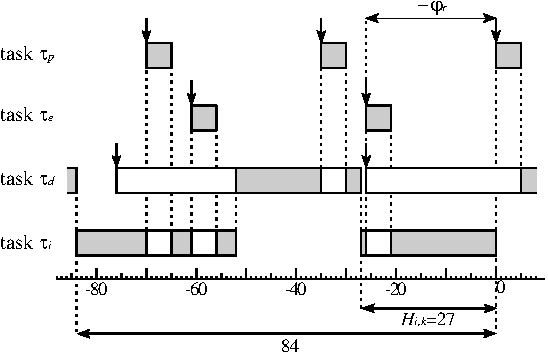
\includegraphics[width=0.5\linewidth]{figures/ex_general_interval1} &
	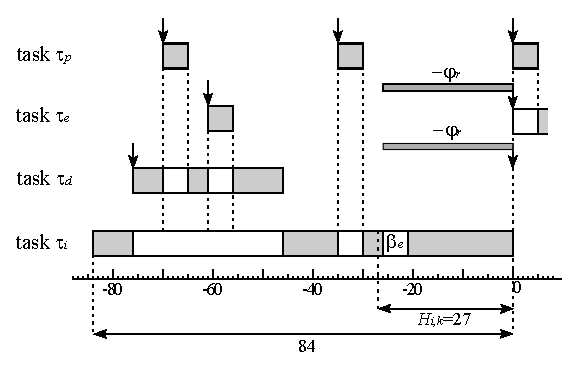
\includegraphics[width=0.5\linewidth]{figures/ex_general_interval2}
	\end{tabular}
	
	\caption{Two timelines for $\mathpzc{T}_{\ref{tab:ex_general_interval}}$ depicting the \textit{generalized best-case interval} $GI(2 \cdot BC_i,\mathpzc{E_i}) = 84$, where $\mathpzc{E_i} = \{\tau_e\}$. (a) shows the interval under FPTS scheduling while (b) shows the same interval in the analogous representation using FPPS when injecting an artificial activation jitter of $-\phi_r$ to tasks $\tau_d$ and $\tau_e$.}
	\label{fig:ex_general_interval1}
\end{figure}

Given the notion of \textit{generalized best-case interval}, the \textit{best-case response time} analysis for FPTS follows directly from the analysis for FPPS.

\begin{theorem} \label{thm:bcrt_fpts_1}
	Let $\mathpzc{E}^{br}_i$ be the set of \textit{extra preemptive} tasks of a task $\tau_i\in \mathpzc{T}$ that leads to its best-case response time. Furthermore, let $wl^{\prime}_i$ exists, where $wl^{\prime}_i$ is the worst-case number of jobs of $\tau_i$ in a level-$i$ active period in task-set $\mathpzc{T_i}=\{\tau_a | \pi_a \geq \pi_i, \tau_a \in \mathpzc{T} \}$. The best-case response time of task $\tau_i$ scheduled under FPTS is given by 
	\begin{align}
	BR_i = \max \limits_{1 \leq k \leq wl^{\prime}_i} (GI_i(k \cdot BC_i, \mathpzc{E^{br}_i}) - (k-1)T_i).
	\end{align} 
\end{theorem}

It is worth noting that the number of jobs to explore in order to find the \textit{best-case response time} is given by $wl^{\prime}_i$ in Theorem \ref{thm:bcrt_fpts_1}. Furthermore, $wl^{\prime}_i$ is determined using an auxiliary task-set $\mathpzc{T_i}$ that contains all tasks of $\mathpzc{T}$ with the exception of lower priority tasks of $\tau_i$. The reason for this is that, as was proved elsewhere, lower priority tasks do not influence the \textit{best-case response time} of a task $\tau_i$. Therefore, the \textit{best-case response time} of $\tau_i \in \mathpzc{T}$ is the same as the \textit{best-case response time} of the same task in $\mathpzc{T_i}$. Based on this, we conclude that it is sufficient to explore the worst-case number of jobs of $\tau_i$ in a level-$i$ active period in task-set $\mathpzc{T_i}$ to determine the \textit{best-case response time}.

From Theorem \ref{thm:bcrt_fpts_1}, we also observe that we need the set of \textit{preemptive} tasks $\mathpzc{E}^{br}_i$ in order to find the \textit{best-case response time}. Since determining $\mathpzc{E}^{br}_i$ is non-trivial as we will show in the next section, we propose the following theorem where all possible values for $\mathpzc{E}^{br}_i$ are explored.

\begin{theorem} \label{thm:exact_bcrt}
	 Let all tasks of a set  $\mathpzc{T}$ be strictly periodic and let $wl^{\prime}_i$ exists, where $wl^{\prime}_i$ is the worst-case number of jobs of $\tau_i$ in a level-$i$ active period in task-set $\mathpzc{T_i}=\{\tau_a | \pi_a \geq \pi_i, \tau_a \in \mathpzc{T} \}$. Furthermore, let  $\mathpzc{H_i}^{\prime} = \{\tau_h | \pi_h > \theta_i, \exists \tau_d : \theta_i \geq \pi_d > \pi_i \}$ be the set of preemptive tasks of a task $\tau_i \in \mathpzc{T}$ when at least one delaying task exists. The best-case response time of task $\tau_i$ is given by
	 \begin{align}
	 	BR_i = \min\limits_{\mathpzc{E}\in\mathpzc{\hat{E}_i}}(\max \limits_{1 \leq k \leq wl^{\prime}_i} (GI_i(k \cdot BC_i, \mathpzc{E}) - (k-1)T_i)),
	 \end{align}
	 where $\mathpzc{\hat{E}_i}$ is the set of all possible combinations of $\mathpzc{H^{\prime}_i}$ including the empty set.
\end{theorem}


\subsection{Exact BCRT analysis for FPTS is NP-Hard}

In this section, we show that for some task-sets finding the exact best-case response time of a task scheduled using FPTS is NP-hard.

In FPTS, \textit{delaying} tasks may provoke that the best-case response time of a task $\tau_i$ is assumed when some \textit{preemptive} tasks are activated a sufficiently small amount of time after the start of the job $k^{bcrt}$ of $\tau_i$ that assumes the best-case response time. We denoted this category of tasks as \textit{extra preemptive} because they give rise to extra preemptions in job  $k^{bcrt}$, whereas the \textit{preemptive} tasks that interfere at least as possible with $k^{bcrt}$ are called \textit{best preemptive} tasks. Due to this distinction between \textit{extra preemptive} and \textit{best preemptive} tasks, the main concern to determine the best-case response time of a task is to identify which \textit{preemptive} tasks correspond to which category. In other words, given the set $ \mathpzc{H_i} = \{\tau_h | \pi_h > \theta_i\}$ of \textit{preemptive tasks}, we have to find the set $\mathpzc{E_i} \subseteq \mathpzc{H_i}$ of \textit{extra preemptive} tasks that minimizes the response time of $\tau_i$. The set of \textit{best preemptive} tasks is simply given by $\mathpzc{P_i =  \mathpzc{H_i} \backslash \mathpzc{E_i}}$. In principle, this is an optimization problem; however, in many cases the set $\mathpzc{E_i}$ can only be empty. For instance when the task $\tau_i$ is non-preemptive or when there are no \textit{delaying} tasks, i.e. when $\pi_i = \theta_i$. On the other hand, there are other cases where determining the set of \textit{extra preemptive} tasks is not trivial. Table \ref{tab:np_hard} shows an example of such a nontrivial task-set. As we will show, determining the best-case response time of $\tau_i$ for this and similar cases is NP-hard.

\begin{table}[H]
	\center
	\caption{Task set $\mathpzc{T}_{\ref{tab:np_hard}}$.}
	\label{tab:np_hard}
	\begin{tabular}{c c c c c}
		\hline 
		task & $T_i$ & $WC_i=BC_i$ & $\pi_i$ & $\theta_i$ \\ 
		\hline 
		$\{ \tau_{h1},\tau_{h_2},\tau_{h_3},\tau_{h_4},\tau_{h_5} \}$& $\{35,...,35\}$  & $\{3.3,2.3,2,1.3,1.1\}$  & $\{7,...,3\}$ & $\{7,...,3\}$ \\ 
		$\tau_d$& 50 & 20 & 2 & 2 \\ 
		$\tau_i$& 70 & 22 & 1 & 2 \\
		\hline 
	\end{tabular}
	\small
	\item The \textit{least common multiple} of the periods is 350 and $U^{\mathpzc{T_{\ref{tab:np_hard}}}}=1$.
\end{table}

Figure \ref{fig:np_hard1} shows a timeline for $\mathpzc{T}_{\ref{tab:np_hard}}$ where all \textit{preemptive} tasks $\mathpzc{H_i}$ are activated simultaneously with the completion of the last job $\iota_{i,1}$ of $\tau_i$ at time $t=0$. Hence, in this timeline the set $\mathpzc{E}_i$ is empty and the response time of the last job $\iota_{i,1}$ is $R_{i,1}=36$. Furthermore, note that $R_{i,1}$ cannot be reduced by pushing the activations of $\tau_i$ because  the job $\iota_{i,3}$ activated at time $t=-176$ starts upon activation. Hence, pushing the activation of $\tau_i$ would modify the schedule. In order to reduce the response time of $\iota_{i,1}$, the activations of $\tau_d$ should be pushed to an earlier moment in time till one of its activations occurs at time $t=-176$. In this way, $\tau_d$ will prevent job $\iota_{i,3}$ to start upon activation and, consequently, it will be possible to reduce $R_{i,1}$. However, forcing $\tau_d$ to be activated at time $t=-176$ would lead to an activation of $\tau_d$ at time $t=-26$ as well. In order to avoid this activation to influence on the response time of $\iota_{i,1}$, its hold time has to be increased till $H_{i,1} > 26$.

\begin{figure}[H]
	\centering
	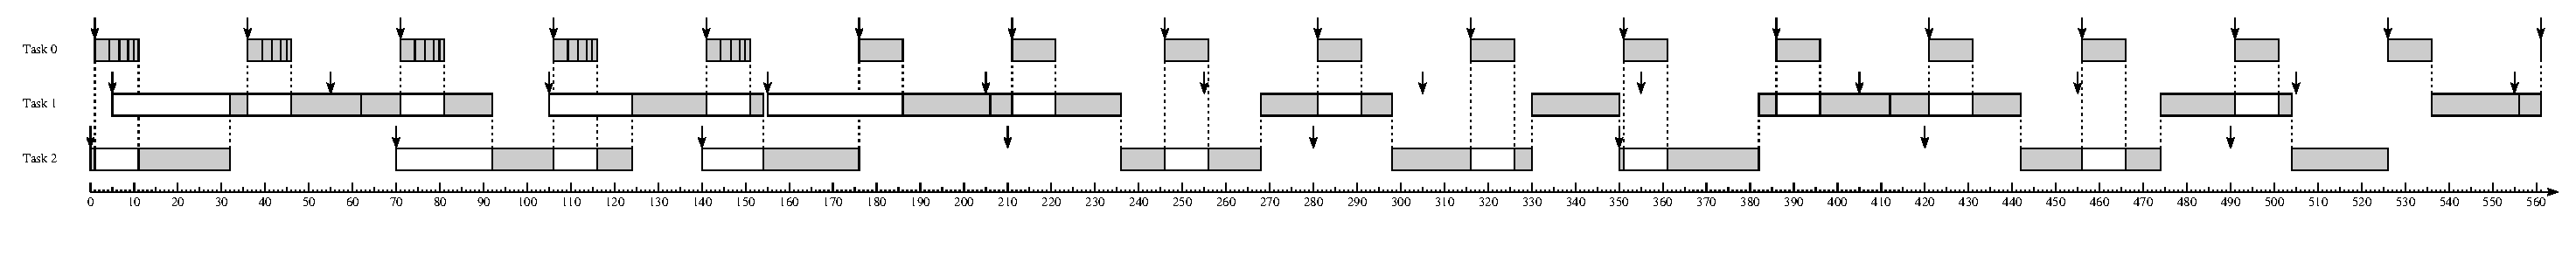
\includegraphics[width=1\linewidth]{figures/multiple_tasks}
	\caption{A timeline for $\mathpzc{T}_{\ref{tab:np_hard}}$ when the set of \textit{extra preemptive} tasks $\mathpzc{E}_i$ is empty. Down-arrows with a "star" denote the activations fo $\tau_d$ that would allow to reduce the response time of the last job $\iota_{i,1}$ of $\tau_i$.}
	\label{fig:np_hard1}
\end{figure}

Since the only tasks that can increase the hold time of $\iota_{i,1}$ are the \textit{preemptive} tasks, the problem reduces to find the \textit{preemptive} tasks that minimizes the hold time of  $\iota_{i,1}$ satisfying the constraint $H_{i,1} > 26$. This problem is an instance of the dual of the well known knapsack problem that has been shown to be NP-hard. For task-set $\mathpzc{T}_{\ref{tab:np_hard}}$, the solution of this problem is depicted in Figure \ref{fig:np_hard2}, where the \textit{extra preemptive} tasks that minimize the response time of $\iota_{i,1}$ are $\tau_{h_2}$ and $\tau_{h_3}$. Therefore, the best-case response time of task $\tau_i$ is $BR_i = BC_i+BC_{h2}+BC_{h3} =26.3$.

\begin{figure}[H]
	\centering
	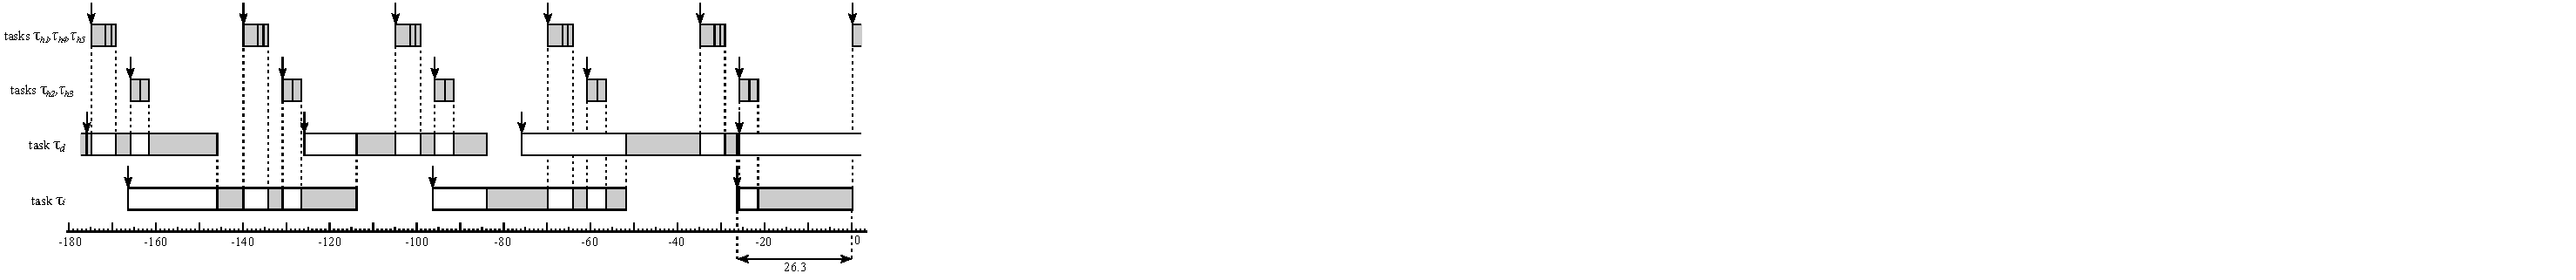
\includegraphics[width=1\linewidth]{figures/multiple_tasks2}
	\caption{A timeline for $\mathpzc{T}_{\ref{tab:np_hard}}$ showing the best-case response time of $\tau_i$ with $BR_i = 26.3$. The set of \textit{extra preemptive} tasks that leads to the best-case response time is $\mathpzc{E}_i=\{\tau_{h_2},\tau_{h_3}\}$.}
	\label{fig:np_hard2}
\end{figure}

\subsection{An algorithm for computing BCRT for FPTS}
The outer $\min$ in the \textit{best-case response time} analysis for FPTS described in Theorem \ref{thm:exact_bcrt} requires to find the minimum response time among all possible combinations of \textit{extra preemptive} tasks. This clearly suggests an algorithm with worst-case time complexity of $\mathcal{O}(2^n)$ for $n$ number of tasks. Due to the inefficient nature of the analysis, in this section we propose an implementation for Theorem 3 that achieves a more tractable complexity on average; however, in the worst-case it is still exponential.

Algorithm 2 shows the exhaustive algorithm to compute the \textit{best-case response time} of a task $\tau_i$ given a task-set $\mathpzc{T}$. The algorithm first calls function $bcrtInit(\mathpzc{T},i)$ to initialize the set of possible \textit{extra preemptive} tasks $\mathpzc{H^{\prime}_i}$ and a first candidate for the \textit{best-case response time} $BR_i$. If $\mathpzc{H^{\prime}_i}$ results to be empty, then the algorithm terminates. Otherwise, the algorithm continues and try to find the minimum response time trying all possible combinations for the set of possible \textit{extra preemptive} tasks.

Algorithm 3 shows the $bcrtInit(\mathpzc{T},i)$ procedure. Line 2 first assigns to $\alpha$ the  best-case hold time when ignoring all \textit{delaying} tasks. Line 3 then checks whether the same hold time can be assumed when introducing \textit{delaying} tasks. If not, the algorithm jumps to Lines 13 and 14 where the set of possible extra preemptive tasks $\mathpzc{H^{\prime}_i}$ is simply initialized with all the \textit{preemptive} tasks. On the other hand, if the hold time can be assumed after introducing \textit{delaying} tasks, there is a high probability that the job experiencing this hold time is the job with the \textit{best-case response time}\footnote{Note: Right now this is just a claim, based on my observations and intuition. Not sure how to support this formally, yet.}. Therefore, the algorithm continues to Line 4 where it computes the shortest response time when there are no \textit{extra preemptive} tasks. In Lines 5-7, it is determined the amount of time that the relative activation $\alpha$ of \textit{delaying} tasks has to be increased in order to reduce the response time. If $\alpha$ results to be greater than the current response time, then there is no way that the response time can be decreased and we indeed have found the \textit{best-case response time}\footnote{Note: Probably this has to be proved as well.}; hence, the set of possible extra preemptive tasks $\mathpzc{H^{\prime}_i}$ becomes empty in Line 9. Otherwise, the \textit{preemptive} tasks that can increase the hold time without exceeding the current response time are added to the set of possible\textit{ extra preemptive} tasks in Line 11.

%\begin{algorithm}[H]
%	\caption{Algorithm to compute hold time given a set of tasks and \textit{extra preemptive} tasks.}\label{euclid}
%	\begin{algorithmic}[1]
%		\Procedure{\textit{computeHoldTime}}{$\mathpzc{T}$,$\mathpzc{E}$,$i$}
%		\State $\mathpzc{P} \gets \{\tau_p | \pi_p > \theta_i, \tau_p \notin \mathpzc{E} \}$;
%		\State $HT_i \gets BC_i; $
%		\State $HT^{old}_i \gets 0$;
%		\State $\beta_p , \beta_e \gets BC_i$;
%		\While {$HT_i > HT^{old}_i$}
%		\State $HT^{old}_i \gets HT_i$;
%		\State $\beta_p \gets HT_i - \beta_e + BC_i$;
%		\State $\beta_e \gets WI_i(\beta_p, \mathpzc{E}) - \beta_p + BC_i$;
%		\State $HT_i \gets BI_i(\beta_e, \mathpzc{P})$;
%		\EndWhile {\textbf{end while}}
%		\If {$HT_i \neq GI_i(BC_i,HT_i,\mathpzc{E})$}
%		\State $HT_i \gets \infty$;
%		\EndIf {\textbf{end if}}
%		\State \Return $HT_i$
%		\EndProcedure
%	\end{algorithmic}
%\end{algorithm}


\begin{algorithm}[H]
	\caption{Exhaustive algorithm to derive \textit{best-case response time} under FPTS.}\label{euclid}
	\begin{algorithmic}[1]
		\Procedure{\textit{bcrtFPTS}}{$\mathpzc{T}$,$i$}
		\State $(BR_i, \mathpzc{H^{\prime}_i}) \gets bcrtInit( \mathpzc{T},i)$;
		\If {$ \mathpzc{H^{\prime}_i} \neq \{\}$}
		\State $\mathpzc{\hat{E}} \gets$ set of all possible combinations of  $\mathpzc{H^{\prime}_i}$;
		\For {\textbf{each} $\mathpzc{E}$ \textbf{of} $\mathpzc{\hat{E}}$}
		\State $BR_i \gets \min\{BR_i, \max \limits_{1 \leq k \leq wl^{\prime}_i} (GI_i(k \cdot BC_i, \mathpzc{E}) - (k-1)T_i)\}$;
		\EndFor {\textbf{end for}}
		\EndIf {\textbf{end if}}
		\State \Return $BR_i$; 
		\EndProcedure
	\end{algorithmic}
\end{algorithm}

\begin{algorithm}[H]
	\caption{Algorithm to derive an initial possible \textit{best-case response time} and a set of candidates of \textit{extra preemptive} tasks.}\label{euclid}
	\begin{algorithmic}[1]
		\Procedure{\textit{bcrtInit}}{$\mathpzc{T}$,$i$}
		\State $\alpha \gets HT_i(\{\})$;
		\If {$\alpha  = GI_i(BC_i, \{\})$}
		\State $BR^{init}_i \gets \max \limits_{1 \leq k \leq wl^{\prime}_i} (GI_i(k \cdot BC_i, \{\}) - (k-1)T_i)$;
		\State $k^{tight} \gets$ the smallest $k$ with $1 \leq k \leq wl^{\prime}_i$ that leads to $BR^{init}_i$;
		\State $DI_i \gets BR^{init}_i + (k^{tight}-1)T_i - \alpha$;
		\State $\alpha \gets \min \{\infty , \min \limits_{d:\theta_i \geq \pi_d > \pi_i} (DI_i \mod T_d)\} + \alpha$;
		\If {$\alpha \geq BR^{init}_i$}
		\State $\mathpzc{H^{\prime}_i} = \{\}$;
		\Else
		\State $\mathpzc{H^{\prime}_i} = \{\tau_h | \pi_h > \theta_i, BC_h < BR_i - \alpha, \tau_h \in \mathpzc{T}\}$
		\EndIf {\textbf{end if}}
		\Else
		\State $BR^{init}_i \gets\infty$; 
		\State $\mathpzc{H^{\prime}_i} = \{\tau_h | \pi_h > \theta_i, \tau_h \in \mathpzc{T}\}$;
		\EndIf {\textbf{end if}}
		\State \Return $BR^{init}_i, \mathpzc{H^{\prime}_i}$; 
		\EndProcedure
	\end{algorithmic}
\end{algorithm}


\begin{thebibliography}{10}
	\bibitem{BLM13}
	R.J. Bril, J.J. Lukkien, and R.H. Mak.
	Best-case response times and jitter analysis of real-time tasks with arbitrary deadlines.
	In Proc. 21st International Conference on Real-Time Networks and Systems (RTNS), ACM, pp. 193-202, October 2013.
	
	\bibitem{BAHDB17}
	R.J. Bril, S. Altmeyer, M.M.H.P. van den Heuvel, R.I. Davis, and M. Behnam.
	Fixed priority scheduling with pre-emption thresholds and cache-related pre-emption delays: integrated analysis and evaluation.
	In Real-Time Systems, 31 January 2017.	
	doi:10.1007/s11241-016-9266-z
	
	\bibitem{BFV08}
	R.J. Bril, G. Fohler, and W.F.J. Verhaegh. 
	Execution times and execution jitter of real-time tasks under fixed-priority preemptive scheduling. 
	Technical Report CSR 08-27, TU/e, The Netherlands, Oct. 2008. \url{http://www.win.tue.nl/~mholende/cantata/publications/BCG-WiP-ECRTS09-final.pdf}
	
	
\end{thebibliography}


\end{document}

